\subsection{Decision Making in IT}

\indent 

\textbf{Decision making} is the \textbf{process of selecting the best possible course of action} from a set of alternatives to achieve a desired goal or solve a problem.

It’s one of the most important skills in professional and organizational contexts, especially in \textbf{Information Technology (IT)}, where choices often have long-term technical, financial, and strategic impacts.

It is important in IT as IT professionals make \textbf{high-impact decisions}, from choosing technologies to managing projects and ensuring data security. \textbf{Data-based decision-making} leads to more \textbf{accurate, transparent, and efficient} outcomes. It reduces bias, supports innovation, and improves risk management.

\begin{figure}[htbp]
    \centering
    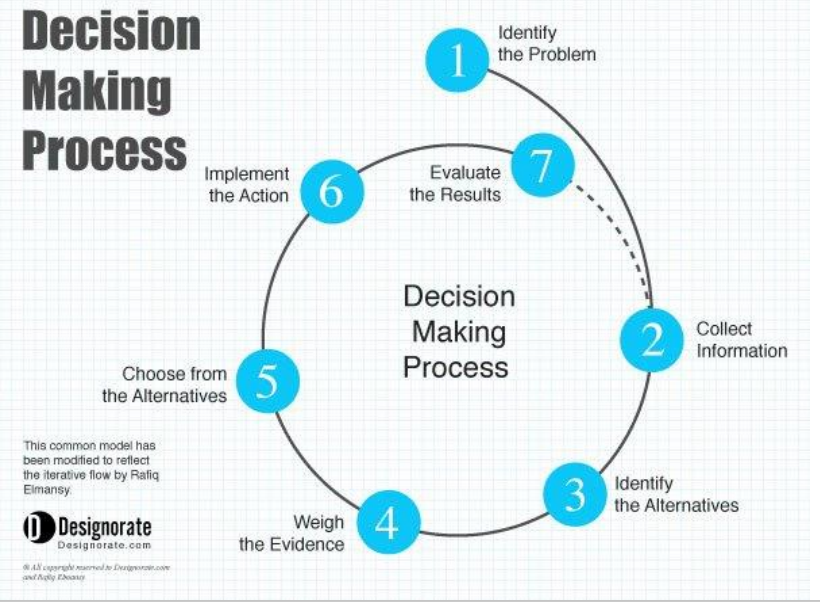
\includegraphics[width=0.7\linewidth]{figures/Week 12/DM Process.png}
\end{figure}

\begin{itemize}
    \item Identify the problem: The first step is to clearly define what needs to be decided or solved.
    \item Collect Information: Gather relevant \textbf{data, facts, and evidence} to understand the problem fully. This can include user analytics, system logs, financial reports, or stakeholder feedback.
    \item Identify the Alternatives: List possible courses of action or solutions. Good decision-making requires creative thinking and multiple options.
    \item Weigh the Evidence: Evaluate each alternative by considering \textbf{pros, cons, risks, and outcomes}. You may use decision matrices, SWOT analysis, or cost–benefit analysis.
    \item Choose from the Alternatives: Select the most suitable solution based on the evidence collected. This step combines \textbf{data-driven reasoning} with \textbf{professional judgment}.
    \item Implement the Action: Put the decision into action. This includes assigning tasks, allocating resources, and setting timelines.
    \item Evaluate the Results: Review the outcomes of the decision to see if it solved the problem or achieved the goal.
\end{itemize}

\subsubsection{Types of Decisions based on the Level of Management}

\indent 

Organisations make decisions at three key management levels:

\begin{itemize}
    \item Operational (Lower-level management): Operational decisions are routine, day-to-day choices that ensure the smooth functioning of an organisation’s ongoing activities. They typically deal with short-term goals and have low risk.
    \item Tactical (Middle management): Tactical decisions are medium-term, project- or department-level decisions that translate strategic goals into practical actions. They are semi-structured, combining data analysis with managerial judgment.
    \item Strategic (Top management): Strategic decisions are long-term, organization-wide decisions that define the direction, vision, and competitive advantage of the company. They are unstructured, high-risk, and have far-reaching consequences.
\end{itemize}

\begin{table}[htbp]
\centering
\renewcommand{\arraystretch}{1.35}
\begin{tabular}{|c|c|c|c|}
\hline
\textbf{Aspect} & \textbf{Operational Decision} & \textbf{Tactical Decisions} & \textbf{Strategic Decisions} \\
\hline

\textbf{Focus} &
Daily operations &
Project execution &
Long term vision \\
\hline

\textbf{Level} &
Supervisors / Technicians &
Manager / Team Leads &
Executives / Directors \\
\hline

\textbf{Time Frame} &
Short Term &
Medium Term &
Long Term \\
\hline

\textbf{Nature} &
Structured &
Semi-Structured &
Unstructured \\
\hline

\textbf{Data Type} &
Transactional, detailed &
Summarised reports &
Aggregated, predictive \\
\hline

\textbf{Risk} &
Low &
Moderate &
High \\
\hline

\end{tabular}
\caption{Types of Decisions Based on Management Levels}
\end{table}

\subsubsection{Rational vs Intuitive Decision Making}

\indent

\begin{table}[htbp]
\centering
\renewcommand{\arraystretch}{1.4}
\begin{tabular}{|c|p{6cm}|p{6cm}|}
\hline
\textbf{Aspect} & \textbf{Rational Decision Making} & \textbf{Intuitive Decision Making} \\
\hline

\textbf{Introduction} &
A logical, structured, and data-driven approach where decisions are made after careful analysis of facts, data, and alternatives. &
A spontaneous, experience-based process that relies on gut feeling, instincts, or professional judgment rather than analytical reasoning. \\
\hline

\textbf{Focus} &
Objectivity, evidence, and reasoning. &
Experience, pattern recognition, and tacit knowledge. \\
\hline

\textbf{Goal} &
Maximize outcomes by minimizing uncertainty through analysis. &
Make timely, confident decisions in uncertain or time-pressured situations. \\
\hline

\end{tabular}
\caption{Comparison of Rational vs Intuitive Decision Making}
\end{table}

\subsubsection{IT Specific Decision challenges}

\indent 

Every IT decision, from choosing a new software tool to designing a cybersecurity strategy, involves balancing \textbf{technical feasibility, business value, user experience, cost, and risk}.

IT decision-making is characterised by:

\begin{itemize}
    \item \textbf{High uncertainty}: due to evolving technologies and unpredictable project outcomes.
    \item \textbf{Complex interdependencies}: as one technical decision often impacts multiple systems or departments.
    \item \textbf{Rapid change cycles}: where decisions made today might need revision in months or even weeks.
    \item \textbf{Multi-stakeholder involvement}: requiring collaboration between technical experts, managers, and end-users.
    \item \textbf{Strong reliance on data}: supported by analytics, performance metrics, and 
predictive models.
\end{itemize}

\subsubsection{1. Rapid technological change}

\indent

Technology evolves faster than organizational policies, budgets, and skill sets can adapt. IT professionals often need to make decisions with \textbf{incomplete or rapidly changing information}.

Challenges:

\begin{itemize}
    \item Short technology lifecycles $\rightarrow$ risk of tools becoming obsolete.
    \item Pressure to adopt new tech (e.g., AI, blockchain, cloud computing) before fully understanding implications.
    \item Balancing innovation with stability.
\end{itemize}

Professional Insight: Use \textbf{technology roadmaps} and \textbf{proof-of-concept (POC)} evaluations to manage uncertainty and reduce risk

\subsubsection{2. Data driven vs Experience driven decision}

\indent 

Modern IT decisions rely heavily on data (metrics, analytics, KPIs), but \textbf{not all factors can be quantified}. Experienced professionals bring intuition and context that data might miss.

Challenges:

\begin{itemize}
    \item Over-reliance on data may ignore human or contextual insights.
    \item Over-reliance on intuition may introduce bias or errors.
    \item Conflicts between analytics teams and senior managers.
\end{itemize}

Professional Insight: The most effective IT leaders combine \textbf{quantitative data} with \textbf{qualitative judgment}.

\subsubsection{3. Security vs Usability trade-offs}

\indent

Every IT system faces a fundamental trade-off between \textbf{tight security} and \textbf{user convenience}. Stronger security often introduces complexity, while simplicity can reduce protection.

Challenges:

\begin{itemize}
    \item Balancing security compliance with user experience.
    \item Justifying security investments with limited budgets.
    \item Managing user resistance to strict controls.
\end{itemize}

Professional Insight: Adopt a \textbf{risk-based security model}, where the level of security matches the sensitivity of the system.

\subsection{Business Intelligence}

\textbf{Business Intelligence (BI)} refers to the \textbf{processes, technologies, and tools} that collect, integrate, analyze, and present \textbf{business data} to help organizations make \textbf{informed, data-driven decisions}.

In simple terms, BI turns \textbf{raw data into actionable insights}, enabling businesses to understand what’s happening, why it’s happening, and what to do next.

In modern organizations, \textbf{data is one of the most valuable assets}. However, data alone has little value unless it can be translated into insights that guide strategy and operations. That’s where \textbf{Business Intelligence} comes in.

\subsubsection{Business Intelligence vs Analytics vs Data Science}

\indent

\begin{table}[htbp]
\centering
\renewcommand{\arraystretch}{1.35}
\begin{tabular}{|p{3cm}|p{4cm}|p{4cm}|p{4cm}|}
\hline
\textbf{Aspect} &
\textbf{Business Intelligence} &
\textbf{Business Analytics} &
\textbf{Data Science} \\
\hline

\textbf{Primary Focus} &
\textbf{Descriptive understanding} – focuses on reporting, monitoring, and summarising existing data to understand \textit{what has happened} in the organisation. &
\textbf{Predictive and prescriptive analysis} – explores data trends, identifies patterns, and forecasts \textit{what is likely to happen or what should be done next}. &
\textbf{Discovery and automation} – uses advanced algorithms and machine learning to uncover hidden patterns and enable automated, data-driven actions. \\
\hline

\textbf{Purpose} &
To provide visibility and transparency into business operations through dashboards and reports. &
To provide deeper insights and strategic guidance by analyzing causes and predicting outcomes. &
To build intelligent systems and data products that can learn, adapt, and make predictions or decisions autonomously. \\
\hline

\textbf{Techniques} &
Reporting, dashboards, OLAP &
Statistical modeling, forecasting &
Machine learning, AI, NLP \\
\hline

\end{tabular}
\caption{Comparison of Business Intelligence, Business Analytics, and Data Science}
\end{table}

\subsubsection{BI Architecture \& Components}

\indent 

\textbf{BI Architecture} is a \textbf{structured framework} that defines how data flows from sources to actionable insights for decision-making. It ensures that \textbf{data is collected, transformed, stored, analyzed, and presented} efficiently to support both operational and strategic decisions. Think of it as the \textbf{pipeline that turns raw data into intelligence}.

\begin{figure}[htbp]
    \centering
    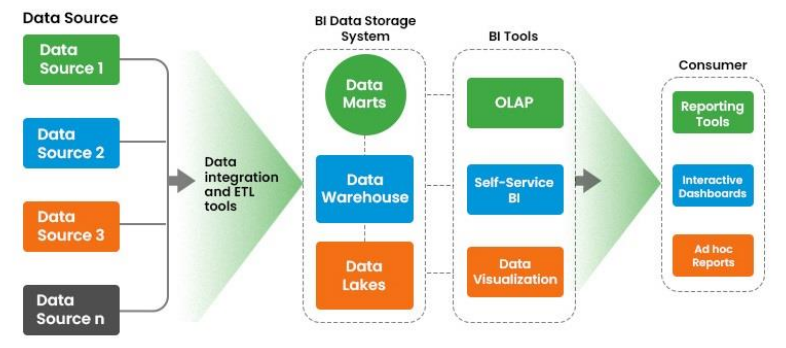
\includegraphics[width=0.8\linewidth]{figures/Week 12/BI Architure.png}
\end{figure}

\subsubsection{How BI supports Decision making?}

\begin{itemize}
    \item Provides Data-driven insights: BI systems collect and consolidate data from multiple sources such as sales, finance, marketing, operations, etc. This unified view eliminates guesswork.
        
        Impact: Managers can base decisions on facts and trends rather than intuition.
    \item Improves Decision speed and accuracy: Real-time dashboards and automated reports allow faster access to performance data.
        
        Impact: Enables timely decisions and proactive responses to business issues.
    \item Identifies trends and opportunities: BI tools use historical and current data to reveal emerging patterns.
        
        Impact: Helps businesses anticipate market changes, customer behavior, and growth opportunities.
\end{itemize}

\subsubsection{BI and IT Decision Challenges}

\begin{itemize}
    \item Data quality and accuracy: BI systems rely heavily on clean and accurate data. Inconsistent, incomplete, or duplicate data leads to misleading insights.
    \item Data integration: Organizations collect data from various systems (ERP, CRM, social media, IoT, etc.). Integrating these into one BI platform is complex.
    \item Data governance and security: BI systems deal with sensitive data that must comply with regulations (GDPR, HIPAA, etc.). Lack of governance leads to unauthorized access or compliance breaches.
    \item System integration with legacy platforms: Many businesses still run legacy systems incompatible with modern BI tools.
\end{itemize}

\subsubsection{Current Trends}


\begin{itemize}
    \item AI and Machine Learning Integration :BI tools are increasingly embedding AI/ML to generate insights, forecasts, and automate analysis. Features like natural-language query (NLQ), automated storytelling, anomaly detection are becoming standard. Organisations are also building \textbf{semantic layers} to make AI-powered BI more accurate and governed.
    \item Self-service BI \& Democratisation of Data: More business users (not just data specialists) are being empowered to explore data, build dashboards, and get insights. Low-code/no-code BI platforms are gaining traction.
    \item Real time analytics \& Edge computing: More use of streaming data, event-driven analytics, processing data at the “edge” (near data source) for low latency. Real-time dashboards and decisioning are increasingly expected.
\end{itemize}

\subsubsection{Future Challenges}

\begin{itemize}
    \item Managing Data explosion and complexity: The volume, velocity, and variety of data are growing exponentially (IoT, social media, sensors, AI models). BI systems must handle \textbf{structured, semi-structured, and unstructured data} at scale.
        
        Challenge: Designing architectures that can efficiently manage \textbf{real-time, multi-source, and massive datasets} without performance loss.
    \item Balancing AI automation with Human oversight: Modern BI increasingly uses AI for predictive and prescriptive analytics. However, \textbf{automated insights without human context} can lead to flawed or biased decisions.
        
        Challenge: Maintaining \textbf{explainability, transparency, and ethical governance} of AI-driven BI systems.
    \item Ensuring Data Ethics, Privacy, and Compliance: Data protection regulations (GDPR, CCPA, Australia’s Privacy Act) are becoming stricter. BI tools must comply while still enabling deep analysis.
        
        Challenge: Balancing \textbf{data accessibility with privacy}, and ensuring \textbf{ethical use} of data insights.
    \item Real-time Decision fatigue: With the rise of real-time analytics, organizations risk \textbf{information overload}. Constant data streams can overwhelm managers, leading to rushed or poor decisions.
        
        Challenge: Designing systems that provide \textbf{contextual, prioritized insights}, not raw data floods.
\end{itemize}

\subsection{BI Architecture}

\subsubsection{Data Sources Layer}

\indent 

The origin of all data. Data can come from multiple \textbf{internal and external sources}, structured or unstructured.

Purpose: Provide \textbf{raw information} for the BI system to process.

Types of Data Sources:

\begin{itemize}
    \item \textbf{Internal Systems}: ERP, CRM, HR systems, financial databases.
    \item \textbf{External Sources}: Social media, market reports, IoT sensors, web APIs.
    \item \textbf{Unstructured Data}: Emails, documents, audio/video files.
\end{itemize}

\subsubsection{ETL Layer (Extract, Transform, Load)}

\indent

ETL is the \textbf{process that collects, cleans, and prepares data} for analysis.

\textbf{Purpose}: Ensure \textbf{data quality, consistency, and usability}.

Steps:

\begin{itemize}
    \item \textbf{Extract}: Pull data from various sources.
    \item \textbf{Transform}: Clean, normalize, aggregate, and structure data.
    \item \textbf{Load}: Store transformed data into a data warehouse or data mart.
\end{itemize}

\subsubsection{Data Warehouse/Data Storage Layer}

\indent 

A \textbf{centralized repository} for storing \textbf{historical and structured data} from multiple sources.

\textbf{Purpose}: Provides \textbf{a single source of truth} for business reporting and analysis.

Key points:

\begin{itemize}
    \item Optimized for \textbf{querying and reporting}.
    \item Supports \textbf{OLAP (Online Analytical Processing)} for multidimensional analysis.
    \item May include \textbf{data marts} for specific departments (e.g., finance, sales, HR)
\end{itemize}

\subsubsection{OLAP \& Analytical Processing Layer}

\indent 

This layer allows \textbf{multi-dimensional data analysis} such as slicing, dicing, drilling down, rolling up, and pivoting, to uncover insights.

\textbf{Purpose}: Enable \textbf{interactive analysis and insights discovery}.

Key Features:

\begin{itemize}
    \item \textbf{Slicing}: View data for a specific dimension (e.g., sales by region).
    \item \textbf{Dicing}: Analyze data across multiple dimensions simultaneously.
    \item \textbf{Drill Down / Roll Up}: Move between detailed and summarized data.
    \item \textbf{Pivot}: Rotate data dimensions for alternative perspectives.
\end{itemize}

\subsubsection{BI Tools/Platforms}

\textbf{Business Intelligence (BI) tools} are software applications that \textbf{collect, process, analyze, and visualize} large volumes of business data to help organizations make data-driven decisions.

\subsection{OLAP Operations}

\subsubsection{Slicing}

\indent 

\begin{figure}[htbp]
    \centering
    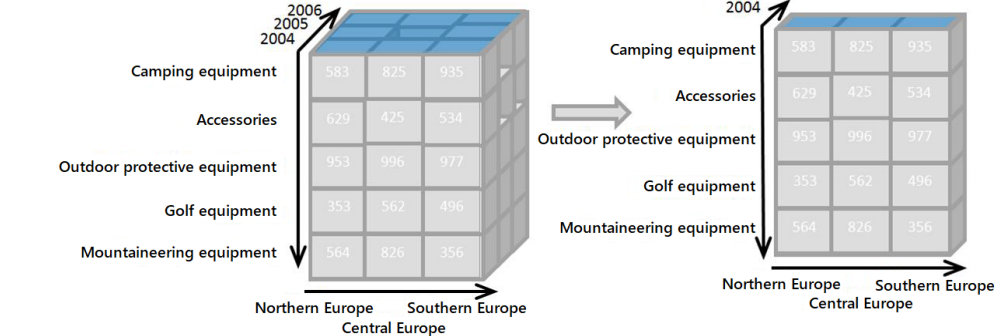
\includegraphics[width=0.8\linewidth]{figures/Week 12/Slicing.png}
    \caption{Slicing}
\end{figure}

Definition: Selects a single layer of data along one dimension of a cube.

Purpose: Focuses on a specific subset of data.

Example: Looking at sales data only for “2025” across all regions and products.

\subsubsection{Dicing}

\indent 

\begin{figure}[htbp]
    \centering
    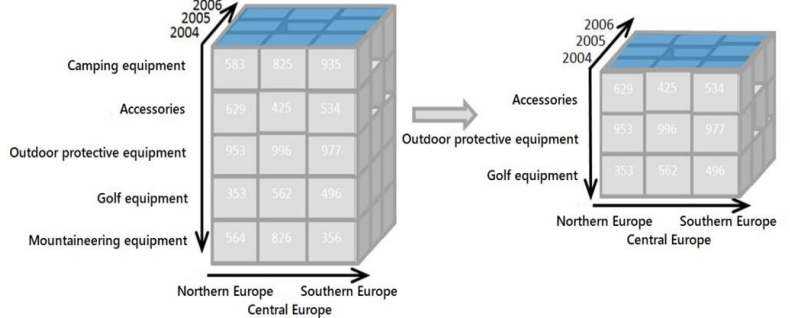
\includegraphics[width=0.8\linewidth]{figures/Week 12/Dicing.png}
    \caption{Dicing}
\end{figure}

Definition: Selects a sub-cube by choosing specific values across multiple dimensions.

Purpose: Analyzes data for multiple criteria at once.

Example: Viewing sales data for Region = Asia and Product = Laptop during Q1 2025.

\subsubsection{Drill Down}

\indent 

\begin{figure}[htbp]
    \centering
    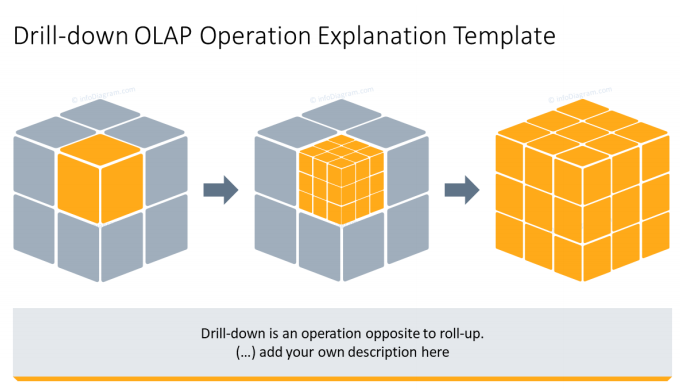
\includegraphics[width=0.6\linewidth]{figures/Week 12/Drill Down.png}
    \caption{Drill Down}
    \label{fig:placeholder}
\end{figure}

Definition: Moves from \textbf{summary data to more detailed data}.

Purpose: Understand granular details behind aggregated results.

Example: From quarterly sales totals to monthly or daily sales.

\subsubsection{Roll up}

\indent 

\begin{figure}[htbp]
    \centering
    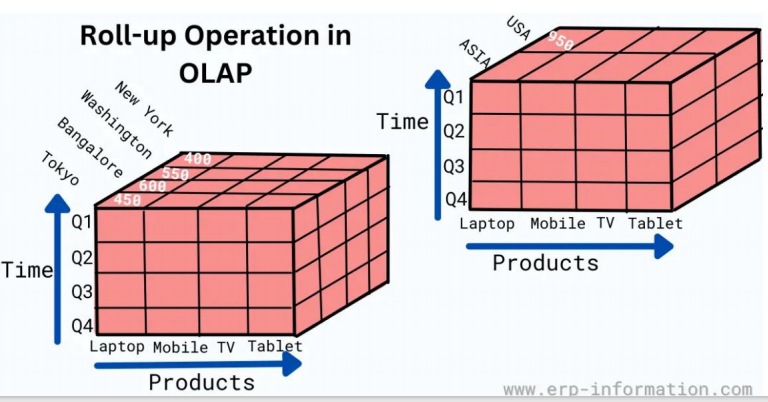
\includegraphics[width=0.7\linewidth]{figures/Week 12/Roll up.png}
    \caption{Roll up}
\end{figure}

Definition: Aggregates data from \textbf{a detailed level to a higher summary level}.

Purpose: Provides high-level overview or trend analysis.

Example: From daily sales → monthly sales → yearly sales.

\subsubsection{Pivot (Rotate)}

\indent 

\begin{figure}
    \centering
    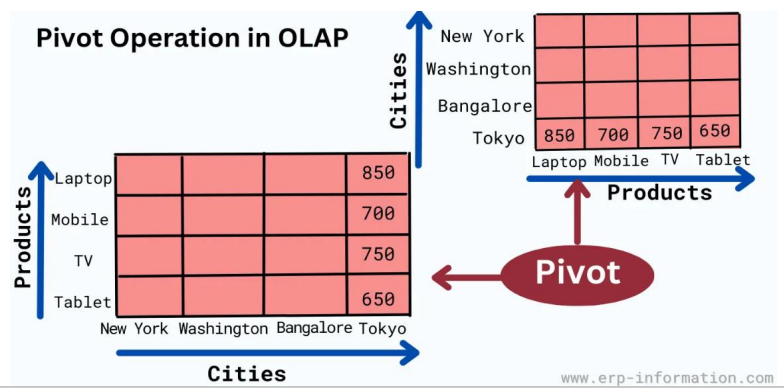
\includegraphics[width=0.7\linewidth]{figures/Week 12/Pivot (Rotate).png}
    \caption{Pivot (Rotate)}
\end{figure}

Definition: Reorients the data cube to \textbf{change the perspective}.

Purpose: Makes it easier to analyze relationships between dimensions.

Example: Swap rows and columns in a report: instead of Region as rows and Product as columns, you show Product as rows and Region as columns.

\subsection{Questions}

\subsubsection{End of Lecture Questions}

\begin{itemize}
    \item What is Business Intelligence (BI), and how does it differ from traditional data reporting?
    \item How does BI contribute to better decision-making across different management levels?
    \item How would you use BI to improve operational efficiency in a retail or healthcare setting?
    \item Define rational and intuitive decision making. In what situations is each approach more effective?
    \item Describe how decision making differs at the operational, tactical, and strategic levels of management.
    \item What strategies can be used to ensure ethical decision making when using AI or automated systems?
\end{itemize}

\subsubsection{Case Study}

\indent 

NovaTech Solutions is a mid-sized IT services company that recently implemented a Business Intelligence (BI) platform to improve its decision-making process.

Previously, departmental managers made decisions based on spreadsheets and personal judgment, leading to inconsistent outcomes. Now, the BI system integrates real-time data from sales, customer feedback, project performance, and financial systems.

During a quarterly review, the BI dashboard revealed that customer satisfaction scores had dropped by 15\% in the last two months. Further analysis showed delays in project delivery and increased staff turnover in the technical support team.

Management must now decide how to address these issues before they impact client retention and profitability

\bigskip

\noindent \textbf{Case Study based Questions}

\begin{itemize}
    \item Identify the type(s) of decision (operational, tactical, or strategic) that management needs to make in this situation. Explain your reasoning.
    \item How can NovaTech use its BI system to analyze the root causes of the declining customer satisfaction scores?
    \item What IT tools or techniques (e.g., dashboards, predictive analytics, data visualization) could help management make informed decisions?
    \item Discuss how a combination of rational and intuitive decision making might be used to solve the problem.
    \item What are two potential challenges NovaTech might face in relying on BI for decision making, and how could they overcome them?
\end{itemize}